% Options for packages loaded elsewhere
\PassOptionsToPackage{unicode}{hyperref}
\PassOptionsToPackage{hyphens}{url}
%
\documentclass[
  ignorenonframetext,
]{beamer}
\usepackage{pgfpages}
\setbeamertemplate{caption}[numbered]
\setbeamertemplate{caption label separator}{: }
\setbeamercolor{caption name}{fg=normal text.fg}
\beamertemplatenavigationsymbolsempty
% Prevent slide breaks in the middle of a paragraph
\widowpenalties 1 10000
\raggedbottom
\setbeamertemplate{part page}{
  \centering
  \begin{beamercolorbox}[sep=16pt,center]{part title}
    \usebeamerfont{part title}\insertpart\par
  \end{beamercolorbox}
}
\setbeamertemplate{section page}{
  \centering
  \begin{beamercolorbox}[sep=12pt,center]{part title}
    \usebeamerfont{section title}\insertsection\par
  \end{beamercolorbox}
}
\setbeamertemplate{subsection page}{
  \centering
  \begin{beamercolorbox}[sep=8pt,center]{part title}
    \usebeamerfont{subsection title}\insertsubsection\par
  \end{beamercolorbox}
}
\AtBeginPart{
  \frame{\partpage}
}
\AtBeginSection{
  \ifbibliography
  \else
    \frame{\sectionpage}
  \fi
}
\AtBeginSubsection{
  \frame{\subsectionpage}
}
\usepackage{lmodern}
\usepackage{amssymb,amsmath}
\usepackage{ifxetex,ifluatex}
\ifnum 0\ifxetex 1\fi\ifluatex 1\fi=0 % if pdftex
  \usepackage[T1]{fontenc}
  \usepackage[utf8]{inputenc}
  \usepackage{textcomp} % provide euro and other symbols
\else % if luatex or xetex
  \usepackage{unicode-math}
  \defaultfontfeatures{Scale=MatchLowercase}
  \defaultfontfeatures[\rmfamily]{Ligatures=TeX,Scale=1}
\fi
% Use upquote if available, for straight quotes in verbatim environments
\IfFileExists{upquote.sty}{\usepackage{upquote}}{}
\IfFileExists{microtype.sty}{% use microtype if available
  \usepackage[]{microtype}
  \UseMicrotypeSet[protrusion]{basicmath} % disable protrusion for tt fonts
}{}
\makeatletter
\@ifundefined{KOMAClassName}{% if non-KOMA class
  \IfFileExists{parskip.sty}{%
    \usepackage{parskip}
  }{% else
    \setlength{\parindent}{0pt}
    \setlength{\parskip}{6pt plus 2pt minus 1pt}}
}{% if KOMA class
  \KOMAoptions{parskip=half}}
\makeatother
\usepackage{xcolor}
\IfFileExists{xurl.sty}{\usepackage{xurl}}{} % add URL line breaks if available
\IfFileExists{bookmark.sty}{\usepackage{bookmark}}{\usepackage{hyperref}}
\hypersetup{
  pdftitle={CSC8631 : Data Management and Explore Data Analysis------Online Learning},
  pdfauthor={Minye Shao},
  hidelinks,
  pdfcreator={LaTeX via pandoc}}
\urlstyle{same} % disable monospaced font for URLs
\newif\ifbibliography
\usepackage{graphicx,grffile}
\makeatletter
\def\maxwidth{\ifdim\Gin@nat@width>\linewidth\linewidth\else\Gin@nat@width\fi}
\def\maxheight{\ifdim\Gin@nat@height>\textheight\textheight\else\Gin@nat@height\fi}
\makeatother
% Scale images if necessary, so that they will not overflow the page
% margins by default, and it is still possible to overwrite the defaults
% using explicit options in \includegraphics[width, height, ...]{}
\setkeys{Gin}{width=\maxwidth,height=\maxheight,keepaspectratio}
% Set default figure placement to htbp
\makeatletter
\def\fps@figure{htbp}
\makeatother
\setlength{\emergencystretch}{3em} % prevent overfull lines
\providecommand{\tightlist}{%
  \setlength{\itemsep}{0pt}\setlength{\parskip}{0pt}}
\setcounter{secnumdepth}{-\maxdimen} % remove section numbering

\title{CSC8631 : Data Management and Explore Data Analysis------Online Learning}
\author{Minye Shao}
\date{2019/11/21}

\begin{document}
\frame{\titlepage}

\begin{frame}{The presentation structure}
\protect\hypertarget{the-presentation-structure}{}

\begin{itemize}
\tightlist
\item
  Project objectives
\item
  Business understanding
\item
  Data Understanding
\item
  Data visualization
\end{itemize}

\end{frame}

\begin{frame}{Project objectives}
\protect\hypertarget{project-objectives}{}

The purpose of this project is to explore and manage data by using R
language to sort out and filter the previously disordered data, and
finally present the data of cyber security to ordinary people in a
visual way,this will make it easier for them to effectively understand
the concepts behind the original data
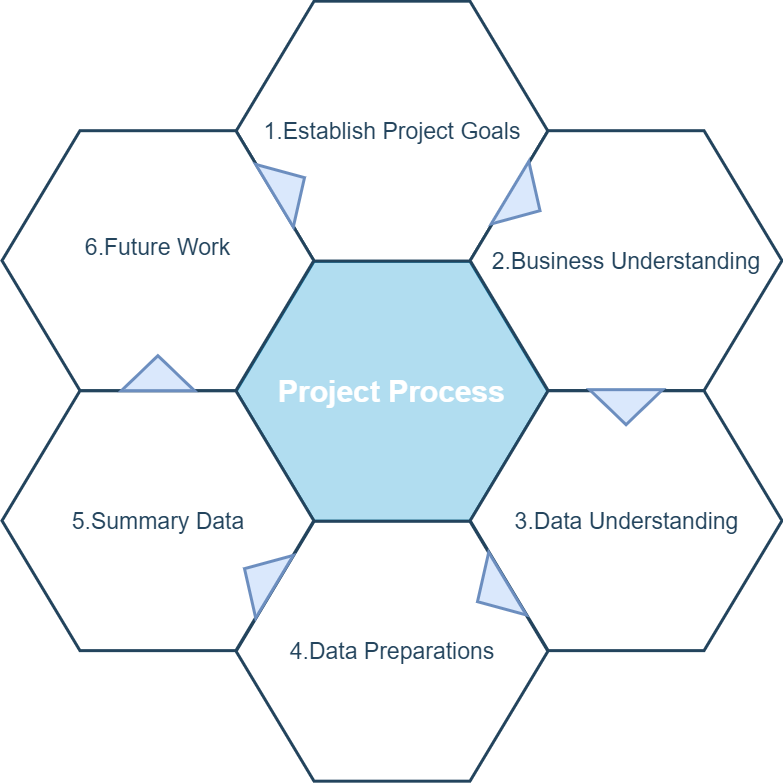
\includegraphics{/CSC8631_CW/Data-Management-CSC8631/new-project/data/Un.png}

\end{frame}

\begin{frame}{Business understanding}
\protect\hypertarget{business-understanding}{}

\begin{itemize}
\tightlist
\item
  With the development of society and science, data analysis and
  processing are more and more widely used.The focus of this project is
  to use the data from the online course of Newcastle university in the
  UK as the prototype, and to draw some effective conclusions by using
  the CRISP-DM model and EDA (exploratory data analysis).Through these
  conclusions, we hope we can improve the course arrangement and
  publicity methods in the future and effectively improve the quality of
  this course.
\item
  We hope that the course of cyber security will be well known and
  everyone can effectively acquire the knowledge they want after
  finishing this course.
\item
  In addition, the study of online courses is more free, with the
  development of the education industry, more and more people will
  choose online courses to study, which is a flexible time choice and
  high-quality education.Therefore, universities can take advantage of
  this opportunity to increase their income.
\end{itemize}

\end{frame}

\begin{frame}{Data Understanding}
\protect\hypertarget{data-understanding}{}

\begin{block}{A basic overview of the data}

\begin{itemize}
\tightlist
\item
  Our data comes from Newcastle university's online course: cyber
  security.
\item
  There are two types of data: static data and fluid data.
\item
  ``Static data'' is data that has traditionally been collected by
  certain institutions, which can be records in universities.
\item
  ``Fluid data'' is collected from everyday activities, such as swiping
  student card and logging into virtual online learning classrooms.
\item
  We have seven terms for the course data, and are ranked from
  cyber\_security 1 to cyber\_security 7, each of which means a new
  cycle for the course. These raw data recorded a lot of necessary and
  meaningful information but it needs to be filtered and processed
  before it can be used.
\end{itemize}

\end{block}

\begin{block}{Defects in the original data}

\begin{itemize}
\item
  There are many null values and Unknown values in the original data. I
  think null values can be properly processed, such as elimination or
  screening, but I will keep Unknown values, because removing Unknown
  values is equivalent to reducing the sample size and affecting the
  authenticity of samples
\item
  Some of the CSV files in the original data don't give me enough
  information to process efficiently
\item
  The raw data itself cannot be directly used as the input values
  presented in the visual diagram. We need to process the data into the
  way we want it to be before screening it to get the diagram we want
\end{itemize}

\end{block}

\begin{block}{Data preprocessing}

\begin{itemize}
\item
  When I look at the given set of raw data, I finally chose 3 of them as
  the main object of processing the data, they are: ``enrolments'',
  ``question response'', and ``step activity''.
\item
  Here are some data preprocessing example: \textgreater{} head(Q2.6) \#
  A tibble: 6 x 12 X learner\_id quiz\_question
  Average.time.in\textasciitilde{} week\_number
  Time.of.first.a\textasciitilde{} Time.of.last.at\textasciitilde{}
  Total.number.of\textasciitilde{} 1 1 005d686d-\textasciitilde{} 1.8.1
  0 1 2018/6/15 14:58 2018/6/15 14:58 1 2 2 005d686d-\textasciitilde{}
  1.8.2 4 1 2018/6/15 14:59 2018/6/15 14:59 2 3 3
  005d686d-\textasciitilde{} 1.8.3 0 1 2018/6/15 15:00 2018/6/15 15:00 1
  4 4 005d686d-\textasciitilde{} 1.8.4 0 1 2018/6/15 15:00 2018/6/15
  15:00 1 5 5 005d686d-\textasciitilde{} 1.8.5 0 1 2018/6/15 15:01
  2018/6/15 15:01 1 6 6 005d686d-\textasciitilde{} 1.8.6 6 1 2018/6/15
  15:02 2018/6/15 15:02 3 \# \ldots{} with 4 more variables:
  The.total.amount.of.time.it.took.to.get.the.problem.right.unit.s. , \#
  The.correct.number , Wrong.number , The.correct.rate.digits.2. 
\item
  Taking ``question\_response.csv'' as an example, through integration,
  we can collect all the answer data under a student id into one piece,
  which will greatly enhance the usability of the original data
\end{itemize}

\end{block}

\end{frame}

\begin{frame}{Data visualization}
\protect\hypertarget{data-visualization}{}

\begin{itemize}
\item
  With data we have processed previously, we can make the following
  chart with shiny.
\item
  By filtering the data, we can obtain the histograms we want. Through
  these histograms, we can obtain the following data:
\end{itemize}

\end{frame}

\end{document}
